$  $% Innehållet i Vasungavisor 2010
%
% Kapitel "Så Härlig Bouquet"

\songchapter{Så Härlig Bouquet}
\begin{figure}[!b]
\begin{center}
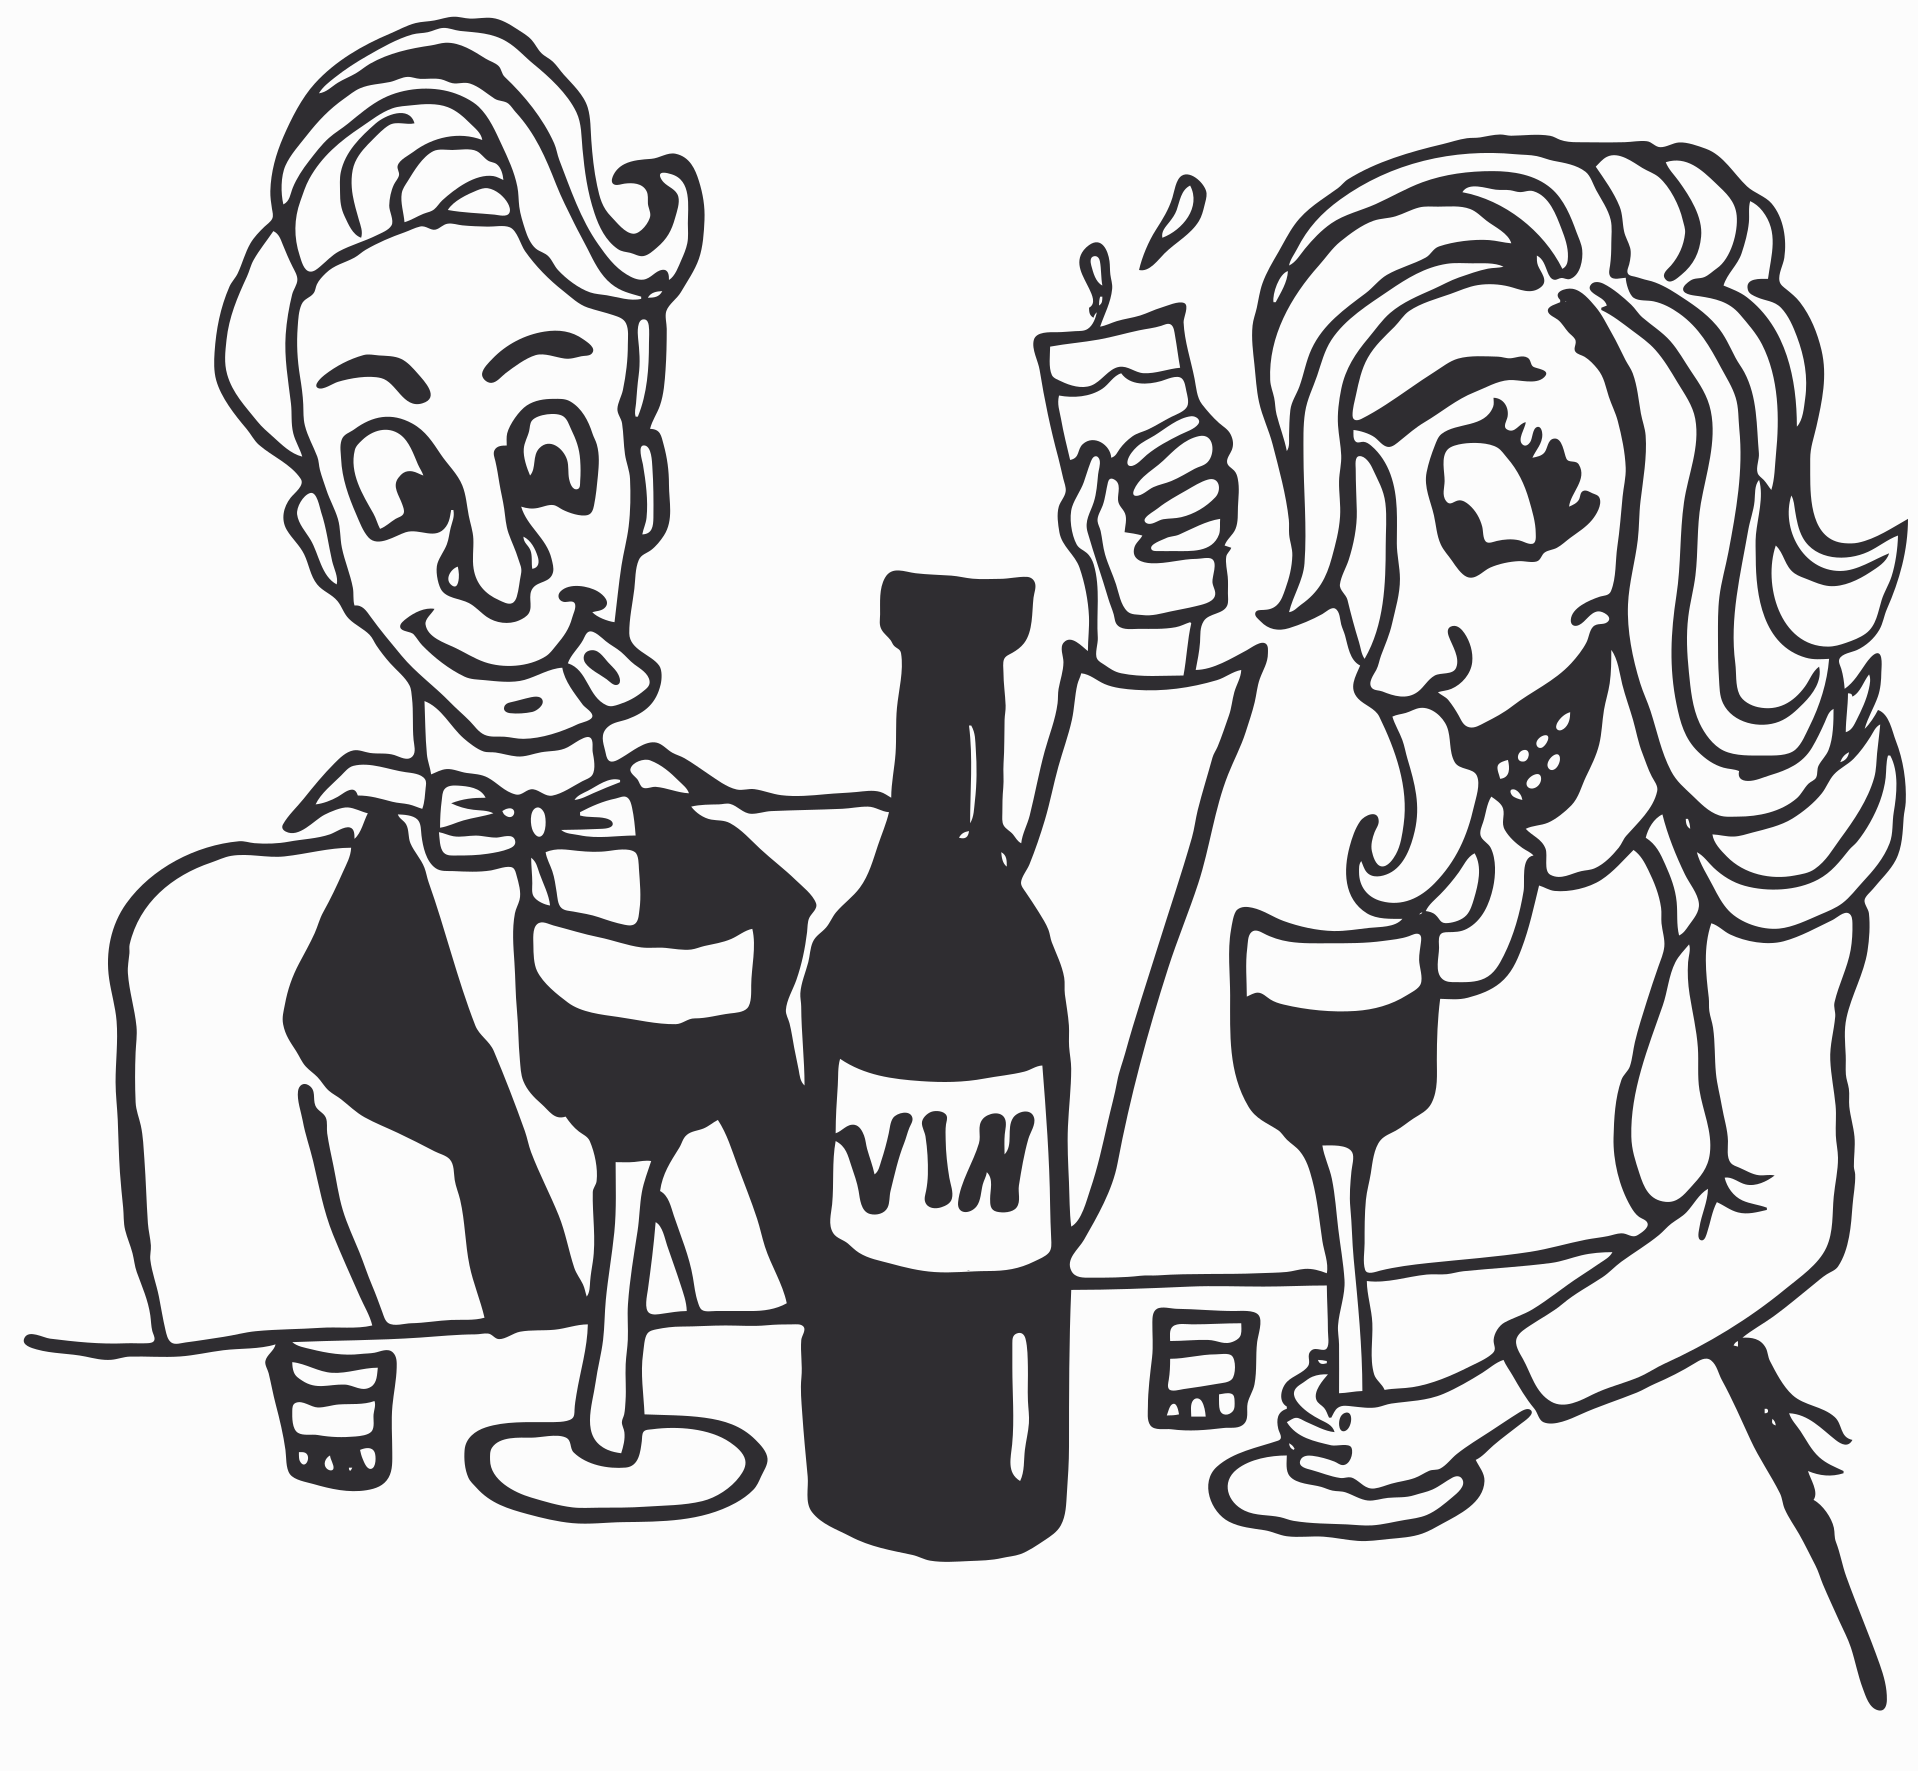
\includegraphics[width=3cm]{../bilder/fardigabilder/BilderTillKapitel/vinvisor.png} 
\end{center}
\end{figure}
\sclearpage
% Sångtext till VN:s sångbok 2018.

% Denna fil kan användas som sådan, bara verserna,
% namnen och annan rådata behöver bytas ur fälten.
% Tecknet "%" markerar en kommentar som helt och 
% hållet ignoreras av programmet som läser filen.

\beginsong{Fredmans sång nr 21}[ 		% Börja sången här
	by={Carl Mikael Bellman},					% Författare
	sr={},					% Melodi
	index={Så lunka vi så småningom}, % Alternativa
	index={Tycker du att graven är för djup}]						% sångnamn
	
\beginverse*						% Börja vers
Så lunka vi så småningom
från Bacchi buller och tumult,
när döden ropar: ''Granne, kom,
ditt timglas är nu fullt!''
Du gubbe, fäll din krycka ner —
och du, du yngling, lyd min lag:
den skönsta nymf som åt dig ler,
inunder armen tag!
\endverse							% Sluta vers

\beginchorus						% Börja refräng
Tycker du att graven är för djup,
nå, välan så tag dig då en sup,
tag dig sen dito en, dito två, dito tre,
så dör du nöjdare!
\endchorus							% Sluta refräng

\beginverse*
Du, vid din remmare och press
rödbrusig och med hatt på sned,
snart skrider fram din likprocess
i några svarta led!
Och du, som pratar där så stort
med band och stjärnor på din rock,
ren snickarn kistan färdig gjort
och hyvlar på dess lock!
\endverse

\beginchorus						% Börja refräng
Tycker du ..
\endchorus							% Sluta refräng

\beginverse*
Men du, som med en trumpen min
bland riglar, galler, järn och lås
dig vilar på ditt penningskrin
inom din stängda bås,
och du, som svartsjuk slår i kras
buteljer, speglar och pokal,
bjud nu godnatt, drick ur ditt glas
och hälsa din rival!
\endverse

\beginchorus						% Börja refräng
Tycker du ..
\endchorus

\beginverse*
Och du, som under titlars klang
din tiggarstav förgyllt vart år,
som knappast har med all din rang
en skilling till din bår,
och du, som ilsken, feg och lat
fördömer vaggan, som dig välvt
och ändå dagligt är plakat
till glasets sista hälft,
\endverse

\beginchorus						% Börja refräng
Tycker du ..
\endchorus

\beginverse*
Du, som vid Martis fältbasun
i blodig skjorta sträckt ditt steg,
och du, som tumlar i paulun,
i Chloris armar feg,
och du, som med din gyllne bok
vid templets genljud reser dig,
som rister huvud, lärd och klok,
och för mot avgrund krig.
\endverse

\beginchorus						% Börja refräng
Tycker du ..
\endchorus

\beginverse*
Och du, som med en ärlig min
plär dina vänner häda jämt
och dem förtalar vid ditt vin,
och det liksom på skämt,
och du, som ej försvarar dem,
fästän ur deras flaskor, du,
du väl kan slicka dina fem,
vad svarar du väl nu?
\endverse

\beginchorus						% Börja refräng
Tycker du ..
\endchorus

\beginverse*
Men du, som till din återfärd,
ifrån det du till bordet gick,
ej klingat för din raska värd,
fastän han ropar: ''Drick!''
Driv sådan gäst från mat och vin,
kör honom med sitt anhang ut
och sen med en ovänlig min
ryck remmaren ur hans trut!
\endverse

\beginchorus						% Börja refräng
Tycker du ..
\endchorus

\beginverse*
Säg, är du nöjd, min grannen, säg!
Så prisa värden nu till slut!
Om vi ha en och samma väg,
så följoms åt... Drick ut!
Men först med vinet, rött och vitt,
för vår värdinna bugom oss —
och halkom sen i graven fritt
vid aftonstjärnans bloss!
\endverse

\beginchorus						% Börja refräng
Tycker du ..
\endchorus

\endsong							% Sluta sång
\sclearpage
% Sångtext till VN:s sångbok 2018.

% Denna fil kan användas som sådan, bara verserna,
% namnen och annan rådata behöver bytas ur fälten.
% Tecknet "%" markerar en kommentar som helt och 
% hållet ignoreras av programmet som läser filen.

\beginsong{Fredmans epistel nr 82}[ 		% Börja sången här
	by={Carl Michael Bellman},					% Författare
	sr={},					% Melodi
	index={Vila vid denna källa}]						% sångnamn

\beginverse*						% Börja vers
Hvila vid denna källa,
Vår lilla Frukost vi framställa;
Rödt Vin med Pimpinella
Och en nyss skuten Beccasin.
Klang hvad Buteljer, Ulla!
I våra Korgar öfverstfulla,
Tömda i gräset rulla,
Och känn hvad ångan dunstar fin,
Ditt middags Vin
Sku vi ur krusen hälla,
Med glättig min.
Hvila vid denna källa,
Hör våra Valdthorns klang Cousine.
[Corno]
Valdthornens klang Cousine.
\endverse							% Sluta vers

\beginverse*						% Börja vers
Prägtigt på fältet pråla,
Än Hingsten med sitt Sto och Fåla,
Än Tjurn han höres vråla,
Och stundom Lammet bråka tör;
Tuppen på taket hoppar,
Och liksom Hönan vingen loppar,
Svalan sitt hufvud doppar,
Och Skatan skrattar på sin stör.
Lyft Kitteln; hör.
Lät Caffe-glöden kola,
Där nedanför.
Prägtigt på fältet pråla
De ämnen som mest ögat rör.
[Corno]
Som mest vårt öga rör.
\endverse							% Sluta vers

\newpage
\beginverse*						% Börja vers
Himmel! hvad denna Runden,
Af friska Löfträn sammanbunden,
Vidgar en plan i Lunden,
Med strödda gångar och behag.
Ljufligt där löfven susa,
I svarta hvirflar grå och ljusa,
Träden en skugga krusa,
Inunder skyars fläkt och drag.
Tag, Ulla tag,
Vid denna måltids stunden,
Ditt glas som jag.
Himmel! hvad denna Runden,
Bepryds af blommor tusen slag!
[Corno]
Af blommor tusen slag! 
\endverse							% Sluta vers

\beginverse*						% Börja vers
Blåsen J Musikanter,
Vid Eols blåst från berg och branter;
Sjungen små Kärleks-Panter,
Bland gamla Mostrars kält och gnag.
Syskon! en sup vid disken,
Och pro secundo en på Fisken;
Krögarn, den Basilisken,
Summerar Taflan full i dag.
Klang Du och Jag!
Klang Ullas amaranther,
Af alla slag!
Blåsen i Musikanter,
Och hvar och en sin kallsup tag.
[Corno]
Hvar en sin kallsup tag.
\endverse							% Sluta vers

\endsong							% Sluta sång
\sclearpage
\input{FredmansSangNr8.tex}
\begin{figure}[!b]
\begin{center}
\includegraphics[width=5cm]{../bilder/flaskor.jpg} 
\end{center}
\end{figure}
\sclearpage
\beginsong{Unkarin viini}[
	by={Carl Michael Bellman, finsk text Reino W. Palmroth}
]
	
\beginverse*						
Voi hyvät ystävät meillä jos ois’
Unkarin viiniä saavi.
Eikö kun kaks’ sitä kantais ja jois’,
paksusti voitais kuin paavi.
Silloinpa veikkoset huolta ei lain,
saavissa kieli kun maattaisiin vain.
Voi hyvät ystävät meillä jos ois’
Unkarin viiniä saavi.
\endverse		

\beginverse*						
Painakoon lyijynä saavimme tuo,
olla ei vaivojen vanki.
Nostava hän, joka laulaa ja juo,
taakan on raskahimmanki!
Veljeni, nyt syliin sieppaan mä sun,
tanssimme ympäri vannehditun.
Voi hyvät ystävät, vuotais nyt vuo,
Oltais ei vaivojen vanki!
\endverse	

\beginverse*						
Ulkona paiste tai pakkanen ei
vaikuta tahtiimme tuimaan.
Ei, vaikka enkelit - hupsis ja hei! - 
loiskaisi saaviimme uimaan.
Lähdön he sais pian pilviä päin,
huutaa ja huitoa jaksamme näin.
Muuta nyt, ystävät, toivota ei:
Päästäispäs saavihin uimaan!
\endverse						
\endsong		

%\sclearpage
%% Sångtext till VN:s sångbok 2018.

% Denna fil kan användas som sådan, bara verserna,
% namnen och annan rådata behöver bytas ur fälten.
% Tecknet "%" markerar en kommentar som helt och 
% hållet ignoreras av programmet som läser filen.

\beginsong{Här är gudagott att vara}[ 		% Börja sången här
	by={Gunnar Wennerberg},					% Författare
	sr={}]						% sångnamn
	
\beginverse*						% Börja vers
Här är gudagott att vara,
o, vad livet dock är skönt!
Hör, vad fröjd från fåglars skara,
se vad gräset lyser grönt.
\endverse							% Sluta vers

\beginchorus						% Börja refräng
Humlan surrar, fjäriln prålar,
lärkan slår i skyn sin drill.
Och ur nektarfyllda skålar
dricka oss små blommor till.
\endchorus							% Sluta refräng
\endsong							% Sluta sång
\begin{figure}[!b]
\begin{center}
\includegraphics[width=5cm]{../bilder/klover.jpg} 
\end{center}
\end{figure}
\sclearpage
% Sångtext till VN:s sångbok 2018.

% Denna fil kan användas som sådan, bara verserna,
% namnen och annan rådata behöver bytas ur fälten.
% Tecknet "%" markerar en kommentar som helt och 
% hållet ignoreras av programmet som läser filen.

\beginsong{När skämtet tar ordet}[ 		% Börja sången här
	by={Frans Mikael Franzén},					% Författare
	sr={},					% Melodi
	index={Frans Mikael Franzéns dryckesvisa}, % Alternativa
	index={Ty en blomma är glädjen}]						% sångnamn
	
\beginverse*						% Börja vers
När skämtet tar ordet vid vänskapens bord,
med fingret På glaset, som dofta,
så drick och var glad: på vår sorgliga jord
man gläder sig aldrig för ofta.
\endverse							% Sluta vers

\beginchorus						% Börja refräng
:: Ty en blomma är glädjen: I dag slår hon ut,
i morgon förvissnar hon redan.
Just nu, då du kan, hav en lycklig minut,
och tänk på den kommande sedan.::
\endchorus							% Sluta refräng

\beginverse*						% Börja vers
Vem drog ej en suck över tidernas lopp?
Dock sitt ej och dröm På kalaset!
Här lev i sekunden, och hela ditt hopp
se fyllas och tömmas i glaset!
\endverse							% Sluta vers

\beginchorus						% Börja refräng
Här sörj blott för glaset: om fyllt, så töm ut;
Om tomt, så försänd det att fYllas,
och minns att det sköna och goda förut,
se'n glädjen och nöjet, må hyllas.
\endchorus							% Sluta refräng

\beginverse*						% Börja vers
Ty ägne vi först åt värdinnan en skål:
vad vore vår fröjd utan henne!
Sen prise vi värden och särskilt hans bål:
vad vore vårt mod utan denne!
\endverse							% Sluta vers

\beginchorus						% Börja refräng
Dem båda förene ett glas och en sång:
de själva så skönt sig förente.
Med druvorna myrten blev skapt på en gång;
vem ser ej, vad himmelen mente?
\endchorus
							% Sluta refräng

\beginverse*						% Börja vers
För övrigt må värden ge alltid nytt skäl
till ständig omsättning på glasen
och visa att rangen är nyttig likväl
till skålarnas mängd på kalasen!
\endverse							% Sluta vers

\beginchorus						% Börja refräng
Men förr'n han är färdig med klang och harang'
vi skynde att självmante dricka
och helge ett glas, som är över all rang'
i tysthet envar åt sin flicka!
\endchorus							% Sluta refräng
\endsong							% Sluta sång
\begin{figure}[!b]
\begin{center}
\includegraphics[width=3cm]{../bilder/vinglas.jpg} 
\end{center}
\end{figure}
\sclearpage
% Innehållet i Vasungavisor 2018

\beginsong{Dricka vill jag vit Chablis}[
  by={Nicklas Forss},
  sr={Plocka vill jag skogsviol}]

\beginverse*
Dricka vill jag vit Chablis och Sachsens fina sekt.
Dricka, dricka, natten lång tills dess min törst är släckt.
Port och Amarone, minna mig om forna dar
och alla flaskor jag i tiden lyckats tömma har.
\endverse

\beginverse*
Dricka vill jag Corvinone, Eiswein och champagne.
Dricka, dricka, Pomerol med färgen av kastanj.
Alla sorters brännvin minna mig om vännen min,
men vinets must åt såna plågor ryter skarpt ``Försvinn!''.
\endverse
\endsong
\sclearpage
% Sångtext till VN:s sångbok 2018.

% Denna fil kan användas som sådan, bara verserna,
% namnen och annan rådata behöver bytas ur fälten.
% Tecknet "%" markerar en kommentar som helt och 
% hållet ignoreras av programmet som läser filen.

\beginsong{Bort allt vad oro gör}[ 		% Börja sången här
	by={Carl Mikael Bellman},					% Författare
	sr={},					% Melodi
	index={Sång nr 17 ur Bacchi Tempel}, % Alternativa
	index={Granne! Gör du just som jag gör}]						% sångnamn
	
\beginverse*						% Börja vers
Bort allt vad oro gör,
bort allt vad hjärtat kväljer!
Bäst att man väljer bland desse buteljer,
sin maglikör.
\endverse							% Sluta vers

\beginchorus						% Börja refräng
Granne! Gör du just som jag gör,
vet denna olja ger humör.
Vad det var läckert!
Vad var det? Rehnskt Bläckert?
Oui, mon seigneur.
\endchorus						% Sluta refräng

\beginverse*						% Börja vers
Bort allt vad oro gör,
allt är ju stoft och aska.
Låt oss bli raska
och tömma vår flaska
bland bröderne.
\endverse							% Sluta vers

\beginchorus						% Börja refräng
Granne! Gör du just som jag gör,
vet denna olja ger humör.
Vad det var mäktigt!
Vad var det?... Jo, präktigt,
Malaga - Ja.
\endchorus


\endsong							% Sluta sång
\sclearpage
% Sångtext till VN:s sångbok 2018.

% Denna fil kan användas som sådan, bara verserna,
% namnen och annan rådata behöver bytas ur fälten.
% Tecknet "%" markerar en kommentar som helt och 
% hållet ignoreras av programmet som läser filen.

\beginsong{Imsig Vimsig}[					% Författare
	sr={Imse vimse spindel}]						% sångnamn
	

\beginverse*						% Börja vers
Imsig vimsig blir man
utav lite vin.
Klättrar uppå stolen,
verkar piggelin.
Ramlar under bordet,
sussar en minut.
Vaknar av att vinet
i glaset tagit slut.
\endverse							% Sluta vers

\endsong							% Sluta sång
%% Sångtext till VN:s sångbok 2018.

% Denna fil kan användas som sådan, bara verserna,
% namnen och annan rådata behöver bytas ur fälten.
% Tecknet "%" markerar en kommentar som helt och 
% hållet ignoreras av programmet som läser filen.

\beginsong{Das Königslied}[ 		% Börja sången här
	by={A.E. Marschner},					% Författare
	sr={},					% Melodi
	index={Ein König ist der Wein}]						% sångnamn
	

\beginverse*						% Börja vers
Ein König ist der Wein, ein König ist der Wein!
Mit Segen reich beladen, ist er von Gottes Gnaden, 
und mancher Purpur sein.
\endverse							% Sluta vers

\beginverse*						% Börja vers
Ein König, ein König, ein König ist der Wein,
Ein König ist der Wein!
\endverse
							% Sluta vers
\beginverse*
Ein König ist der Wein, ein König ist der Wein!
Mit einem Reben bande, umschlingt er alle Lande, 
beherrcht sie gross und klein!
\endverse

\beginverse*
Ein König, ein König, ein König ist der Wein,
Ein König ist der Wein!
\endverse

\vspace{5mm}
\endsong							% Sluta sång
\sclearpage
% Exempel på färdig-formaterad sång till VN:s
% sångbok 2018.

% Denna fil kan användas som sådan, bara verserna,
% namnen och annan rådata behöver bytas ur fälten.
% Tecknet "%" markerar en kommentar som helt och 
% hållet ignoreras av programmet som läser filen.

% Spara den färdiga filen som 
% 'SangnamnUtanMellanslagEllerSkander.tex'
% t.ex. blir "Vid En Källa" till 
% 'VidEnKalla.tex'
% Varje sång blir en egen fil.

\beginsong{Bordeaux, Bordeaux}[ 		% Börja sången här
	by={},					% Författare
	sr={I sommarens soliga dagar},					% Melodi
	index={Jag minns än idag hur min fader}]						% sångnamn
	
\beginverse*						% Börja vers
Jag minns än idag hur min fader 
kom hem ifrån staden så glader
och rada' upp flaskor i rader 
och sade nöjd som så: "Bordeaux, Bordeaux!"
\endverse							% Sluta vers

\beginchorus						% Börja refräng
Han drack ett glas, kom i extas, 
och sedan blev det stort kalas. 
Och vi små glin, ja vi drack vin
som första klassens fyllesvin.
Och vi dansade runt där på bordet
och skrek så vi blev blå:
"Bordeaux, Bordeaux!"
\endchorus							% Sluta refräng

\textnote{Sången sponsoreras av Vasa nations kurator 2018-2020 Azra Arnautovic.}
\endsong							% Sluta sång
\begin{figure}[!b]
\begin{center}
\includegraphics[width=4cm]{../bilder/druvor.jpg} 
\end{center}
\end{figure}
\sclearpage
% Sångtext till VN:s sångbok 2018.

% Denna fil kan användas som sådan, bara verserna,
% namnen och annan rådata behöver bytas ur fälten.
% Tecknet "%" markerar en kommentar som helt och 
% hållet ignoreras av programmet som läser filen.

\beginsong{Feta fransyskor}[ 		% Börja sången här
	by={Okänd författare},					% Författare
	sr={Marsche militaire, Schubert},					% Melodi
	index={Vi vill ha vin}]						% sångnamn
	

\beginverse*						% Börja vers
Feta fransyskor som svettas om fötterna
de trampar druvor som sedan skall jäsas till vin
Transpirationen viktig e’
ty den ger, fin bouquet
Vårtor och svampar följer me’
men vad gör väl de’?
För...
\endverse							% Sluta vers

\beginchorus						% Börja vers
Vi vill ha vin, vill ha vin, vill ha mera vin
även om följderna bli att vi må lida pin
Flickor: Flaskan och glaset gått i sin
Pojkar: Hit med vin, mera vin
Flickor: Tror ni att vi är fyllesvin?
JA! (Fast större)
\endchorus							% Sluta vers
\endsong							% Sluta sång
\begin{figure}[!b]
\begin{center}
\includegraphics[width=50mm]{../bilder/fetfransyska.jpg} 
\end{center}
\end{figure}
\sclearpage
%% Sångtext till VN:s sångbok 2018.

% Denna fil kan användas som sådan, bara verserna,
% namnen och annan rådata behöver bytas ur fälten.
% Tecknet "%" markerar en kommentar som helt och 
% hållet ignoreras av programmet som läser filen.

\beginsong{Nattvarden}[ 		% Börja sången här
	by={},					% Författare
	sr={We are all the winners},					% Melodi
	index={Snabba på med vinet}]						% sångnamn
	

\beginverse*						% Börja vers
Snabba på med vinet
söla inte präst
Strunta i oblaten, nu så är det fest
Skynda, fram med kalken
skit i orgelbrus och sång
Nu sa ska vi ägna oss åt Nattvard dagen lång
\endverse							% Sluta vers

\vspace{5mm}
\endsong							% Sluta sång
% Sångtext till VN:s sångbok 2018.

% Denna fil kan användas som sådan, bara verserna,
% namnen och annan rådata behöver bytas ur fälten.
% Tecknet "%" markerar en kommentar som helt och 
% hållet ignoreras av programmet som läser filen.

\beginsong{Upptappad bakom en vagn}[ 			% Börja sången här
	by={Från ldealkarnevalen 2002},			% Författare
	sr={Visa vid vindens ängar},				% Melodi
	index={Det går ett vin runt med servitrisen}]						% sÃ¥ngnamn
	
\beginverse*

Det går ett vin runt med servitrisen
det porlar till i ett glas med fot.
Och jag skall skramla med bordsservisen
tills det är min tur att ta emot.
Jag ville sjunga om Vino Tinto
och tralla gott om Tokai och Port
men ack, mitt sångblad har jag spillt vin på
och grannens visbok har kommit bort.
Det går ett vin ner för våra strupar
det täpper till våran glada trall.
Men fast jag glömt varje sång om supar
så vill jag sjunga i alla fall,
\endverse

\endsong							% Sluta sång
\sclearpage
\begin{figure}[!b]
\begin{center}
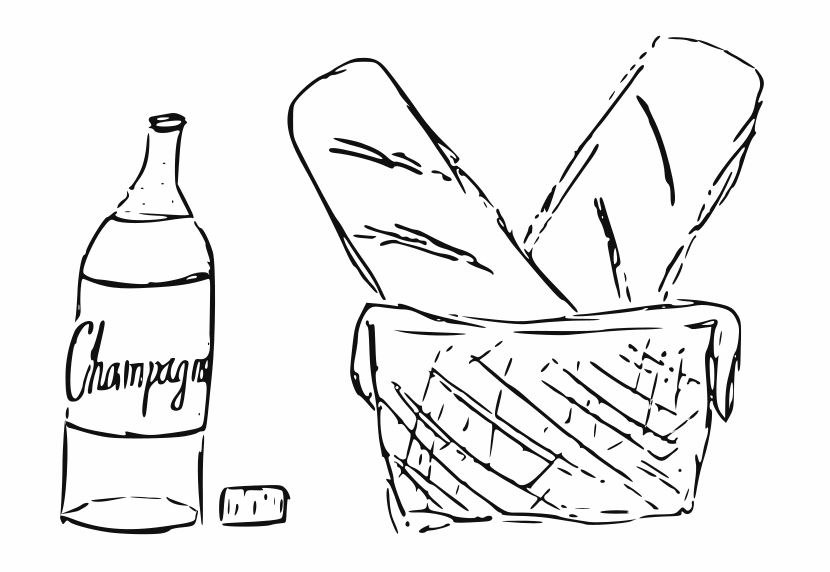
\includegraphics[scale=0.5]{../bilder/batongochvin.png} 
\end{center}
\end{figure}
% Exempel på färdig-formaterad sång till VN:s
% sångbok 2018.

% Denna fil kan användas som sådan, bara verserna,
% namnen och annan rådata behöver bytas ur fälten.
% Tecknet "%" markerar en kommentar som helt och 
% hållet ignoreras av programmet som läser filen.

% Spara den färdiga filen som 
% 'SangnamnUtanMellanslagEllerSkander.tex'
% t.ex. blir "Vid En Källa" till 
% 'VidEnKalla.tex'
% Varje sång blir en egen fil.

\beginsong{Frippes vinvisa}[ 		% Börja sången här
	by={T. Perret},					% Författare
	sr={My Bonnie},					% Melodi
	index={Ett litet glas rödvin mot flunssan}, % Alternativa
	index={Batong och vin}]						% sångnamn
	
\beginverse*						% Börja vers
Ett litet glas rödvin mot flunssan. 
Förbannat så härlig bouquet!
När ungdomen hånglas i Brunssan 
är minnena här ska ni se
\endverse							% Sluta vers

\beginchorus						% Börja refräng
Batong och vin,
rojsigt fint.
Vi skålar med glasen i klang,
champagne!
En kväll på stan, ser man på fan
det är ju Spitu i sin nya BMW, Cabriolet.
\endchorus							% Sluta refräng

\beginverse*						% Börja vers
Med musslor och vin på Hangö västra
i vår Nyländer Yachts ’45.
Med Gusi vi havet bemästra
det mojnar och snart styr vi hem.
\endverse							% Sluta vers

\beginchorus						% Börja refräng
Batong och vin,
rojsigt fint,
vi skålar med glasen i klang,
champagne!
En kväll på stan, ser man på fan
det är ju Spitu i sin nya BMW, Cabriolet.
\endchorus							% Sluta refräng

\beginverse*						% Börja vers
Vi tar å shoppar lite potis från Hallen,
vi kör en brekkare med potatis och sill.
Å har ni hört att Missen har skilt sig
från Nallen?
Å Brassen har fått en klepp till. (ÅTER)
\endverse							% Sluta vers

\beginchorus						% Börja refräng
Batong och vin, rojsigt fint
vi skålar med glasen i klang,
champagne!
En kväll på stan, ser man på fan
Det är ju Gusi som kommer, så skoj,
sidu moj'n!
\endchorus							% Sluta refräng

\vspace{5mm}
\endsong							% Sluta sång
